\documentclass[11pt]{article}
%\documentclass[review]{elsarticle}
\usepackage[utf8]{inputenc}

\usepackage{lmodern}
\usepackage{subfig}
\usepackage[english]{babel}
\usepackage{multirow}
%\usepackage{amsmath,amssymb,psfrag, amsthm}
\usepackage{amsmath,amssymb,psfrag}
\usepackage{graphicx}
\usepackage{fullpage}
\usepackage{listings}
\usepackage{paralist}
\usepackage{appendix}
\usepackage{amsfonts}
\usepackage{subfig,color}
\usepackage{comment} 
\usepackage{enumerate}
\usepackage{cancel}
\usepackage{helvet}
\usepackage{epstopdf}
\usepackage{tikz,tikz-cd}
\usepackage{pgfplots,pgfplotstable}
\usepackage{lineno,hyperref}
\usepackage{mathtools}
\usetikzlibrary{pgfplots.groupplots}
\usetikzlibrary{positioning}
\usetikzlibrary[shapes,arrows,trees]
\usetikzlibrary{matrix,decorations.pathmorphing}
\newcommand{\refalg}[1]{Algorithm~\ref{#1}}
\newcommand{\refsec}[1]{Section~\ref{#1}}
\newcommand{\reffig}[1]{Figure~\ref{#1}}
\newcommand{\refsubfig}[1]{Figure~\subref{#1}}
\newcommand{\reftab}[1]{Table~\ref{#1}}
\newcommand{\refeqn}[1]{(\ref{#1})}
%\newcommand{\reflst}[1]{Listing~(\ref{#1})}


%\newcommand{\refalg}[1]{\cref{#1}}
%\newcommand{\refsec}[1]{\cref{#1}}
%\newcommand{\reffig}[1]{\cref{#1}}
%\newcommand{\refsubfig}[1]{\cref{#1}}
%\newcommand{\reftab}[1]{\cref{#1}}
%\newcommand{\refeqn}[1]{\cref{#1}}
%\newcommand{\reflst}[1]{\cref{#1}}
\renewcommand{\d}{\mathrm{d}}
\newcommand{\re}[1]{(\ref{#1})}
\newcommand{\D}{\mathrm{D}}
\newcommand{\bb}[1]{\boldsymbol{#1}}
\def\sgn{\mathop{\rm sgn}}
\newcommand{\remark}[1]{{\color{red} #1}}
% THEOREMS ETC
\newcommand{\vect}[1]{\mathbf{#1} }
\newcommand{\order}[1]{\mathcal{O}(h^{#1})}
\newcommand{\code}[1]{{\tt #1}}
\renewcommand{\familydefault}{\sfdefault}
% -----------------------------------------------------------
% -----------------------------------------------------------
\lstset{backgroundcolor=\color[rgb]{0.92,0.95,1}}
\lstset{rulecolor=\color[rgb]{0.92,0.95,1}}
\lstset{numbers=left}
\lstset{basicstyle=\ttfamily\footnotesize}
\lstset{numberstyle=\footnotesize}

\def\dfdd#1#2{\frac{\partial#1}{\partial#2}}
\newcommand{\erf}{\, \mathrm{erf}}
\newcommand{\erfc}{\, \mathrm{erfc}}
%\renewcommand{\labelenumi}{[\arabic{enumi}]}
\modulolinenumbers[5]

%\normalsize

\begin{document}
%\def\thefigure{\arabic{figure}}
%\def\thetable{\arabic{table}}

\title{Fourier Neural Networks and how to train them}
\author{Marieme Ngom, Oana Marin \footnote{and ..whoever else takes interest}}
\maketitle
\begin{abstract}

\end{abstract}


%\begin{keyword}
%\texttt{elsarticle.cls}\sep \LaTeX\sep Elsevier \sep template
%\MSC[2010] 00-01\sep  99-00
%\end{keyword}


\linenumbers

\section{Introduction}
% In this work, we solve a variety of PDEs using what we call a deep spectral network. There is extensive work in the literature on how to solve PDEs with machine learnig techniques. In particular Raissi (cite), Sirignano et al. (cite) have proposed deep learning algorithms that aim at solving PDEs. Raissi, Long have proposed algorithms that learn PDEs from data. In Raissi, automatic differentiations are used to approximate the derivatives of the functions produced by the NN. Sirignano et al. use Monte Carlo to perform the second  derivatives and Long et al. make use of convolutions and differential operators to solve the PDEs. 

The last few years have seen revolutionary advances in machine learning techniques in particular through deep learning. The rising availibility of data through data collecting initiatives and technologies have made the use of machine learning ubiquitous in fields like image recognition and finance. Recently (\cite{Raissi}, \cite{Sirignano}), deep learning algorithms have been used to not only solve Partial Differential Equations but also to find the often not known underlying dynamics followed by collected data. Raissi (\cite{Raissi}, Sirignano et al. (\cite{Sirignano}) have proposed deep learning algorithms that aim at solving PDEs. In Raissi, automatic differentiations are used to approximate the derivatives of the functions produced by the neural network. Sirignano et al. use Monte Carlo to perform the second  derivatives. T. Dockhorn (\cite{Dockhorn}) wrote a comprehensive discussion on how to solve the Poisson equation and the steady state Navier-Stokes equation based on the work of Raissi and of Sirignano. Having prior information on the equations to be solved can be used to improve the performance of the neural network.\\

In this work, we are interested in finding periodic solutions to differential equations using neural networks. Periodic solutions of differential equations occur naturally for example for equations in electronics or oscillatory systems. Some differential equations also have periodic boundary conditions which can lead to periodic solutions. To look for periodic solutions one often look for solutions in the form of Fourier series. 
We make use of this and use what is called a Fourier Neural Network which is a neural network with a single hidden layer with activation functions in the form of sine or cosine functions. Fourier Neural Networks were introduced by Gallant and White (\cite{Gallant}) and Silvescu (\cite{Silvescu}), Liu (\cite{Liu}) have also proposed Fourier based networks. Gallant and white use a squashed cosine which allows them to approximate any function depending on the number of nodes in their hidden layer by using Barron's theorem (\cite{Barron}) which says that any function can be approximated by a neural network with a single layer with sigmoidal activation functions. Silvescu and Liu use non sigmoidal activation functions but have given cases where their network perform better than the usual neural networks with sigmoidal activation functions.\\

In this paper, we introduce a new Fourier Neural network that mimics the Fourier decomposition of a periodic function and proves that it can approximate any such functions. We use our network to solve partial differential equations with periodic solutions. \\

The rest of the paper is as follows, first we show how we construct our FNN and how it approximates any periodic function, then we show practical results on approximating certain periodic functions. Finally we use the constructed network to solve PDEs with periodic solutions.





\section{Construction of the Fourier Neural Network}
A neural network can be seen as a function approximator with a number $M$ of inputs, a number $N$ of hidden layers that are composed of nodes and a number $L$ of outputs. In this work, we consider single layer neural networks. The output $\hat{u}$ of a single layer neural network (figure \ref{fig:NN_single}) can be written as
\begin{equation}\label{NN}
  \hat{u_l}(x) = \phi_0 + \sum_{k = 1}^N \lambda_{lk} \sigma\left(\sum_{j = 1}^M w_{kj}x_j + \phi_k \right), \;\; l=1 \cdots N
\end{equation}
where $\{x\}_{j = 1}^M$ are the inputs, $w$ and $\lambda$ are the weights of the neural network, $\sigma$ the activation function, and $\phi$ the biases. One critical component of a neural network is its activation functions. Barron (\cite{Barron}) has proved that any function could be approximated by a single layer neural network with sigmoidal activation functions i.e with an activation function $\sigma$ s.t $\sigma(x) -> 0$ when $x -> -\infty$ and $\sigma(x) -> 1$ when $x -> \infty$. Leshno et al. \cite{Leshno} have proved that multilayer feedforward (define) networks with a nonpolynomial activation function can approximate any function. \\
\begin{figure}[htb]
    \centering
    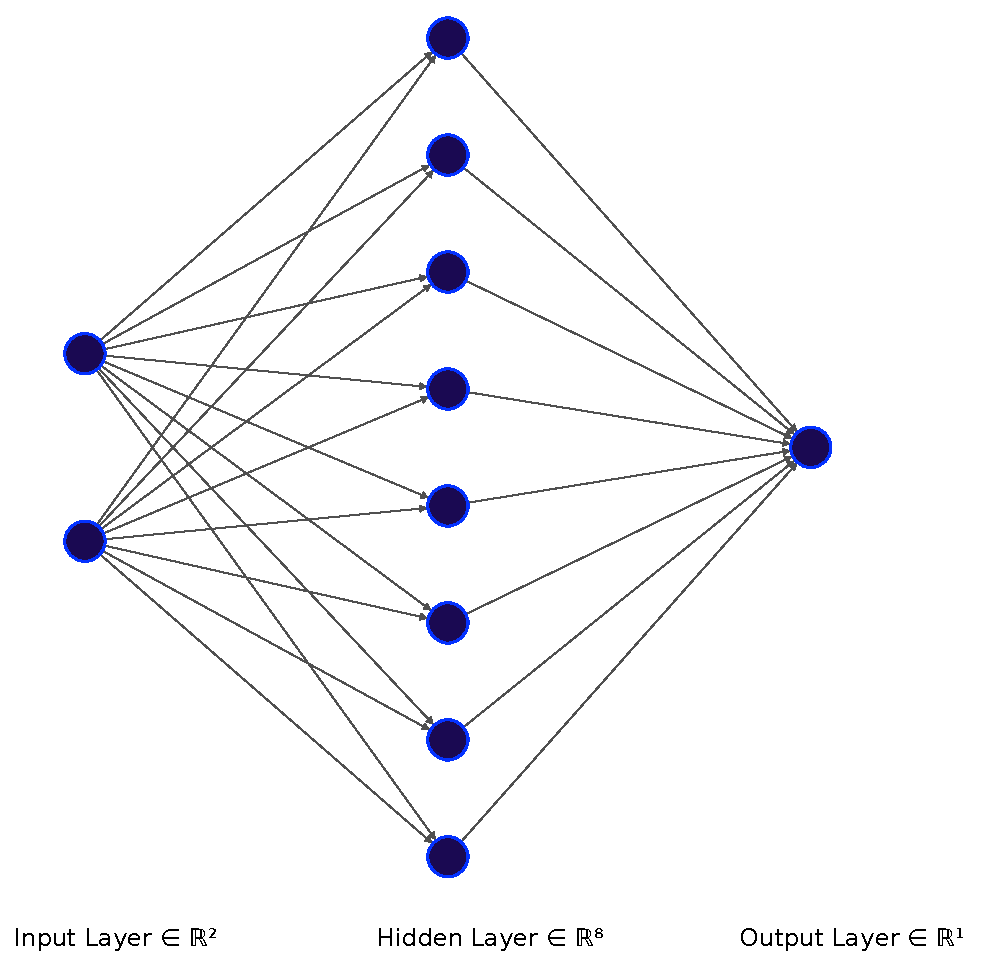
\includegraphics[width=0.45\textwidth]{nn.eps}
    \caption{Fully connected neural network with a single hidden layer}
    \label{fig:NN_single}
\end{figure}
Here, we make use of the Fourier representation $S_N u$ of a T-periodic function $u$ in $L^2(\mathbf R^M)$ which is defined as
\begin{equation}\label{fourier}
    S_{N}u(x) = \sum_{\nu \in \mathbf{N}^M, \nu_{i}\leq N} a_{\nu} \cos(\omega (\nu\cdot x)) + b_{\nu} \sin(\omega(\nu\cdot x)) 
\end{equation}
where $\omega = 2\pi/T$ and $a_{\nu}$ and $b_{\nu}$ the Fourier coefficients of $u$. 
% If we define for $n \geq 1$ $c_{\nu} = \sqrt{a_{\nu}^2 + b_{\nu}^2}$ and $\psi_n = arctan2(-b_{nu}/a_{\nu})$, we can rewrite the above decomposition as
% \begin{equation}\label{fourier_shift}
%     S_N u(x) = \frac{a_0}{2} + \sum_{\nu \in \mathbf{N}^M, \nu_{i}\leq N} c_{\nu} \cos(\omega (\nu\cdot x) + \psi_{\nu})
% \end{equation}
\subsection{The one dimensional case}
In the case where $x \in \mathbf R$, the Fourier approximation is simplified to
\begin{equation}\label{fourier_shift_1d}
    S_N u(x) = \frac{a_0}{2} + \sum_{n=1}^N c_{n} \cos(n \omega x + \psi_{n})
\end{equation}
where $c_{n} = \sqrt{a_{n}^2 + b_{n}^2}$ and $\psi_n = \arctan2(-b_{n},a_{n})$. The function $\arctan2$ is defined as follows:
\begin{equation}
  \arctan2(y, x) = 
    \begin{cases}
      \arctan(y/x) & \text{if $x>0$}\\
      \arctan(y/x)+\pi & \text{if $x<0$ and $y>0$ }\\
      \arctan(y/x)-\pi & \text{if $x<0$ and $y<0$ }\\
      \pi/2 & \text{if $x=0$ and $y>0$ }\\
      -\pi/2 & \text{if $x=0$ and $y<0$ }\\
      undefined & \text{if $x=0$ and $y=0$ }
    \end{cases}       
\end{equation}
For simplicity, we suppose $a_n >0$ to show the equivalency of the two forms of the Fourier series. We have, $$c_{n} \cos(n \omega x + \psi_{n}) = c_{n}\left(\cos(n \omega x) \cos(\psi_{n}) - \sin(n \omega x) \sin(\psi_{n})\right)$$
And, using the fact that $$\cos(\arctan2(-b_{n},a_{n})) = \frac{1}{\sqrt{1+(\frac{b_n}{a_n})^2}}$$
and
$$\sin(\arctan2(-b_{n},a_{n})) = \frac{\frac{-b_n}{a_n}}{\sqrt{1+(\frac{b_n}{a_n})^2}}\; ,$$

we have for $n \geq 1$ 
\begin{align*}
    c_{n} \cos(n \omega x + \psi_{n}) &= \sqrt{a_{n}^2 + b_{n}^2}\left(\cos(n \omega x) \frac{1}{\sqrt{1+(\frac{b_n}{a_n})^2}} - \sin(n \omega x) \frac{\frac{-b_n}{a_n}}{\sqrt{1+(\frac{b_n}{a_n})^2}}\right)\\
   &= \sqrt{a_{n}^2 + b_{n}^2}\left(\cos(n \omega x) \frac{a_n}{\sqrt{a_n^2+b_n^2}} - \sin(n \omega x) \frac{- b_n}{\sqrt{a_n^2+b_n^2}}\right) \\
   &= a_n\cos(n \omega x) +b_n \sin(n \omega x) \\
\end{align*}

\subsubsection{Loss function}
Inspired by the above representation, we construct our network as a one input, one hidden layer with $N$ neurons and one output network with the activation function $\sigma$ being $\sigma(x) = \cos(x)$. Therefore, our output is 
$$ \hat{u}(x) = \phi_0 + \sum_{k = 1}^N \lambda_k \cos\left( w_{k}x + \phi_k. \right)$$
 The goal of our network is to approximate the Fourier approximation $S_N u$ of $u$. To that end, we define our loss function as
 \begin{equation}\label{lossfunction}
     L(\phi, w, \lambda) = ||\hat{u} - u ||^2  + \alpha_1||\lambda||^2 + \alpha_2||w||^2
 \end{equation}
 where
 \begin{enumerate}
     \item The first term ensures that the output of the neural network approximates the target function $u$,
     \item The second and third terms are regularization parameters to avoid overfitting of the Neural Network.
 \end{enumerate}
 
 However, this loss function will not quite give us an approximation of the Fourier series unless we are approximating cosine or sine functions. For example, trying to fit $u(x) = x^2$ with one neuron in the hidden layer led to the output 
 $$\hat{u}(x) = \phi_0 - \lambda_1 \cos(w_1 x)$$ where  $\lambda w_1^2 /2! \approx 1$, $\lambda_1 \approx \phi_1$ and $w_1^{2l} << 1$ for $l >1$. While this, using the fact that
 $$
 \cos(w_1 x) = \sum_{l=1}^{\infty} (-1)^l\frac{w_1^{2l}x^{2l}}{(2l)!} = 1 -w_1^2x^2/2 + o(w_1^3)
 $$
 is a good approximation of $x^2$ is not the our desired result. To get the Fourier representations of our target functions, the weights from the input to the hidden layer need to be integers. This can be achieved by solving a mixed integer optimization problem or by adding a penalty function to the loss which is the route we chose. Our loss function is now
  \begin{equation}\label{lossfunction_good}
     L(\phi, w, \lambda) = ||\hat{u} - u ||^2  + \alpha_1||\lambda||^2 + \alpha_2||w-nint(w)||^2
 \end{equation}
 where $nint(w)$ is the nearest integer to $w$.
\subsubsection{Results}
 We initialize the input to hidden layer weights from a uniform distribution between $0$ and $32$ and the hidden layer to output weight from a uniform distribution between $-pi$ and $+\pi$. First we tried to obtain the learned Fourier Series of $f(x) = x$
 \begin{figure}[!htb]
    \centering
    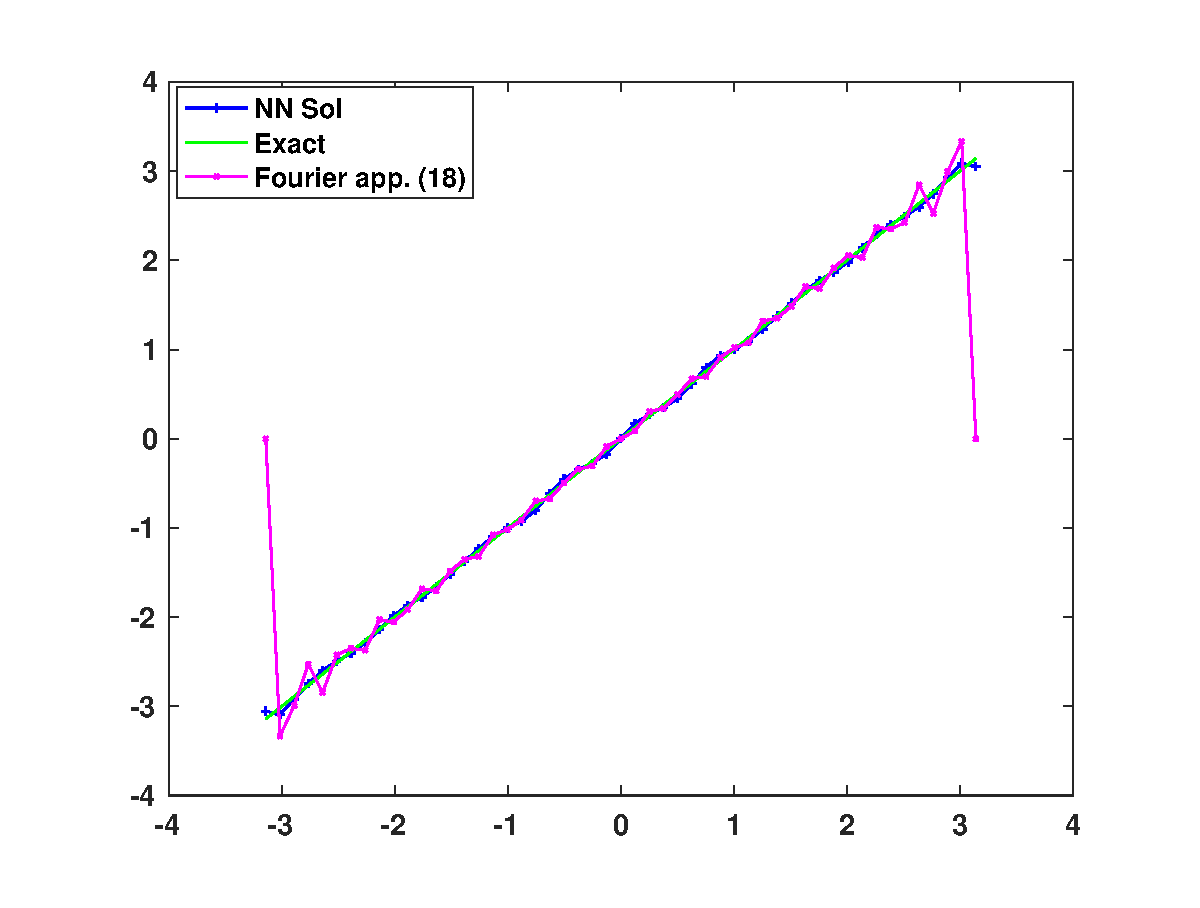
\includegraphics[width=0.5\textwidth]{FourvsNNvsEx_x.eps}
    \caption{Comparison between the approximation obtained by our NN, the $18$ terms Fourier approximation and the exact solution $f(x) = x$.}
    \label{fig:fourvsNN_x}
\end{figure}
 
 

\subsection{The multidimensional case}
In order to approximate equation (\ref{fourier_shift}), we construct the network with $M$ inputs and write the output as
$$ \hat{u}(x) = \phi_0 + \sum_{k = 1}^N \lambda_k \cos\left( w_k\cdot x + \phi_k. \right)$$
and use the same loss function as before. In this case, one need more neurons in the hidden layer in order to skip less $\nu$ in equation \ref{fourier_shift} as possible. 
\subsection{Weights and biases initialization}
It is common practice to initialize the biases of a neural network at $0$ and the weights using a Xavier initialization (\cite{xaviergorot}) or a He initialization (\cite{heinit}). \cite{Kumar} also proposed a weight initialization for activation functions differentiable at zero or not but with biases initialized at zero. When initializing the weights of a neural network, one would like to have $$var(x_{i+1}) = \sigma_{i+1}^2 = var(x_{i}) = \sigma_{i}^2$$.




 \subsection{Results}
 In order to retrieve the Fourier series of $u$, we train our neural network with the loss function
 \begin{equation}\label{loss}
    L(\phi, w, \lambda) = \sum_{k = 1}^N |\hat{u}(x_k) - u(x_k)|^2
 \end{equation}
where $\{x_k\}_{k=1}^{N}$ is the training data that is uniformly drawn in $[\pi/2, \pi/2]$

To validate the model, we first try to recover $u: x -> \cos(x)$ with one neuron in the hidden layer and compare the results with a network trained with the sigmoid and hyperbolic tangent functions. 
Our neural network converges after $85$ iterations and give $$\hat{u}(x) = -\cos(-x + 3.14159265 ) + -1.29629469e-17 \approx -\cos(-x + \pi) = \cos(x) $$.
Using the sigmoid function with $N = 10$ nodes converged in $3516$ iterations and hyperbolic tangent in $2696$ iterations. Furthermore, using a cosine activation function with a Xavier intialization, converges to a loss value of $.68$ which is quite big(\textbf{Put it in a table}).




Then, we try to fit the periodic $u: x -> x^2$ on $[-\pi, \pi]$


\section{Solving PDEs with the constructed Fourier Neural Network}
Instead of using the loss function \ref{MSE}, we use 
 \begin{equation}\label{MSE_pde}
     L = MSE (L\hat{u} - f)
 \end{equation}

\begin{eqnarray*}
    Lu(x) &=& f(x) \;\; in\\
    u(0) &=& u(L)
\end{eqnarray*}
using Neural Networks. 

and then we learn PDEs of the form 
\begin{eqnarray*}
    Lu(t,x) &=& f(t,x)\\
    u(0,x) &=& u_0
\end{eqnarray*}
where $Lu = F(t,x,u,\Delta u, \cdots)$, $x \in R^n$.


\section{Results}



\section{Conclusion}




















\textbf(Multiple hidden layers: First one uses sin/cos activation functions, following uses Relu/sigmoid etc?)
\textbf(Make us of convolutions?)
\textbf(Use Differentiation matrices?(Chebyshev))


The goal of this work is to learn periodic solutions of partial differential equations using a Fourier based Neural Network. More specifically, we will use a neural network with one hidden layer and with an activation function in the form of Fourier basis. We then compare our results to the one obtained from neural networks using sigmoid and reLU activation functions.

PUT FIGURE OF NN WITH FOURIER BASIS AND SHOW HOW THEY APPROXIMATE ANY L2 PERIODIC  FUNCTION

\textbf{Tentative Algorithm}
\begin{itemize}
\item First, compress the data using DCT plus mode selections
\item Second, Use Chebychev Differentiation matrices
\item Third, Apply ML

\end{itemize}




\bibliographystyle{plain}
\bibliography{bie}
\end{document}

%  which looks like the Fourier series of $u$. Hence the goal of our network is to find weights $w$ and biases $\phi$ that equate the fourier coefficients $c_n$ and phase shift $\psi_n$. Obviously, for trigonometric functions, one would need a fewer nodes in the hidden layer than for other functions. For example, one would expect our neural network to converge to the solution quickly if the function to be learned is $\cos(x)$ and to only need one neuron in the hidden layer. To avoid using too many or too few neurons in the hidden layer,  we use a dynamical approach. We start with a hidden layer with one neuron and add neurons as the optimization unfold.



%  \subsection{Weights and biases initialization}
%  It is common practice to initialize the biases of a neural network at $0$ and the weights using a Xavier initialization (\cite{xaviergorot}) or a He initialization (\cite{heinit}). \cite{Kumar} also proposed a weight initialization for activation functions differentiable at zero or not but with biases initialized at zero. When initializing the weights of a neural network, one would like to have $$var(x_{i+1}) = \sigma_{i+1}^2 = var(x_{i}) = \sigma_{i}^2$$. Here we initialize the biases ${\phi_i}_{i=0}^{N}$ uniformly on $[\pi/2, pi/2]$ i.e $\phi_i~ U([-pi/2, pi/2])$. That means the expectation $\mu(\phi_i) = 0$ and $var(\phi_i) = \pi^2/12$. We also suppose that the inputs ${x_0(j)}_{j=1}^M$ are uniformly drawn on $[-\pi, \pi]$. Thetrefore, $\mu(x_j) = 0$ and $var(x_0(j)) = \sigma_i = \pi^2/3.$ Additionnaly, we assume the weights $\lambda_{kj}$ are drawn from a normal distribution with mean $0$ and variance $v^2$ and the $w_k$ from a normal distribution with mean $0$ and variance $\omega^2$. The goal is to find $v^2$ and $\omega^2$ s.t $$var(x_{i+1}) = \sigma_{i+1}^2 = var(x_{i}) = \sigma_{i}^2$$.\\
 
%  From the form of our network, we have for the neurons in the hidden layer and using taylor approximations, we have
%  \begin{equation}
%      x_1{i} \approx \cos(\phi^1_i) + y_0(1)(-\sin(\phi^1_i))
%  \end{equation}
%  where $y_0(1) = \sum_{j=1}^M \lambda_{1j}x_0(j)$. From this, we have $\mu(y_0(1)) = 0$ and $var(y_0(1)) = M* v^2 * pi^2/3$.
% Therefore, $\mu(x_1{i}) = \mu(\cos(\phi^1_i))$. Using the law of the unconscious statistician, we have 
% \begin{align*}
%     \mu_1 = \mu(x_1(i)) = \mu(\cos(\phi^1_i)) &= \int_{0}^{\pi/2} \frac{1}{\pi}\cos(\phi^1_i)  + \int_{-\pi/2}^{0} -\frac{1}{\pi}\cos(-\phi^1_i)\\
%     &= \int_{0}^{\pi/2} \frac{1}{\pi}\cos(\phi^1_i)  + \int_{0}^{\pi/2} \frac{1}{\pi}\cos(-\phi^1_i)\\
%     &= \int_{0}^{\pi/2} \frac{1}{\pi}\cos(\phi^1_i)  + \int_{0}^{\pi/2} \frac{1}{\pi}\cos(\phi^1_i)\\
%     &= 2\int_{0}^{\pi/2} \frac{1}{\pi}\cos(\phi^1_i) \\
%     &=  \frac{2}{\pi}
% \end{align*}
% where we have used the fact that $\cos(-x) = cos(x)$.
% For the variance, we have
% \begin{align*}
%     s_1^2 = var(\cos(\phi^1_i)) + \mu(y_0^2(i))\mu(\sin^2(\phi^1_i)) - \mu(y_0^(i))^2\mu(\sin(\phi^1_i))^2
% \end{align*}
%  We use again the law of the unconscious statistician and obtain
%  \begin{align*}
%     \mu(\sin^2(\phi^1_i)) = \mu(1 - \cos^2(\phi^1_i)) = 1 - \mu(\sin^2(\phi^1_i)) = 1 -1/2 = 1/2
% \end{align*}
% Therefore,
% \begin{align*}
%     s_1^2 = 1/2 - (2/pi)^2 + M* v^2 * pi^2/6
% \end{align*}
% We want $s_1^2 = \pi^2/3$ so, we have the following equation for $v^2$
% \begin{equation*}
%     \pi^2/3 = 1/2 - (2/pi)^2 + M* v^2 * pi^2/6
% \end{equation*}
% which means
% \begin{equation}
%     v^2 = \frac{6}{M\pi^2}\left(\pi^2/3 - 1/2 +4/\pi^2 \right)
% \end{equation}
% Now, for the output, we have
% \begin{equation*}
%     x_2 = \sum_{i =1}^N w_i x_1(i) + \phi_0
% \end{equation*}
% So that 
% \begin{align*}
%     \mu(x_2) &= \sum_{i =1}^N \mu(w_i) \mu(x_1(i)) + \mu(\phi_0) \\
%         &= \mu(\phi_0) = 0
% \end{align*}
% and
% \begin{align*}
%     s_2^2 &= \sum_{i =1}^N \left(\mu(w_i^2) \mu(x_1^2(i))-  \mu^2(w_i) \mu^2(x_1(i))\right) + var(\phi_0) \\
%         &= N\omega^2(s_1^2 - \mu_1^2) + var(\phi_0)\\
%         & = N\omega^2(\frac{\pi^2}{3} - \frac{4}{\pi^2}) + var(\phi_0)
% \end{align*}
% Again, we want $s_2^2 = \frac{pi^2}{3}$. To achieve that, we initialize the output bias at $0$ so that $var(\phi_0) = 0$ and set
% \begin{equation}
%     \omega^2 = \frac{\pi^2}{3N(\pi^2/3 - 4/\pi^2)}
% \end{equation}
